% Propósito: mostrar que una octava puede dividirse en tres tercios contiguos
% sobre un eje logarítmico y que el ancho absoluto crece con la frecuencia.
% Origen: ecuaciones f_L=f_c 2^{-1/(2b)}, f_H=f_c 2^{1/(2b)} y B=f_H-f_L.
% Para la octava centrada en 1000 Hz: límites 707,1 y 1414,2 Hz.
% Los tres tercios tienen centros 793,7; 1000 y 1259,9 Hz, límites comunes
% 707,1; 890,9; 1122,5; 1414,2 Hz y anchos 183,8; 231,6; 291,8 Hz.
% Esquema matemático sobre eje logarítmico; no representa filtros medidos.
% Descripción accesible: una barra superior abarca la octava de 707,1 a
% 1414,2 Hz alrededor de 1000 Hz. Debajo, tres barras contiguas ocupan el mismo
% intervalo sobre el eje logarítmico. Aunque tienen la misma razón entre
% límites, sus anchos en hertz aumentan hacia frecuencias más altas.
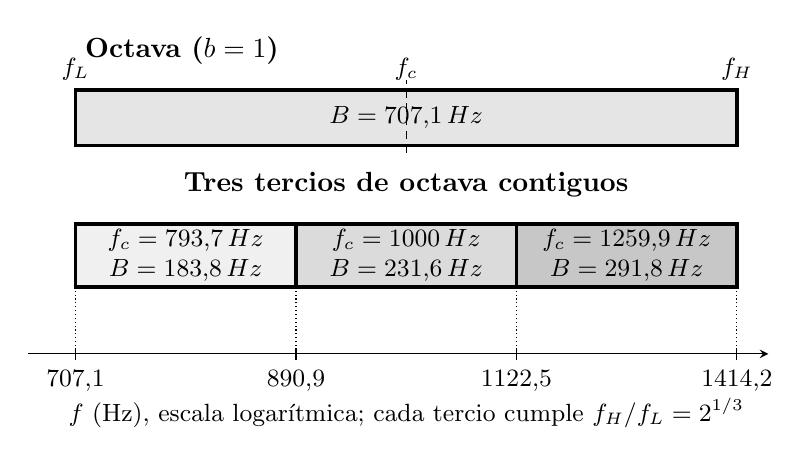
\begin{tikzpicture}[font=\small,>=stealth,x=1cm,y=1cm]
    \node[anchor=west,font=\bfseries] at (1.40,4.55)
        {Octava (\(b=1\))};

    \draw[fill=black!10] (1.40,3.35) rectangle (9.80,4.05);
    \draw[very thick] (1.40,3.35) rectangle (9.80,4.05);
    \draw[densely dashed] (5.60,3.25) -- (5.60,4.18);
    \node at (5.60,3.70) {\(B=707{,}1\,\text{Hz}\)};
    \node[above] at (1.40,4.05) {\(f_L\)};
    \node[above] at (5.60,4.05) {\(f_c\)};
    \node[above] at (9.80,4.05) {\(f_H\)};

    \node[font=\bfseries] at (5.60,2.85)
        {Tres tercios de octava contiguos};
    \draw[fill=black!6] (1.40,1.55) rectangle (4.20,2.35);
    \draw[fill=black!14] (4.20,1.55) rectangle (7.00,2.35);
    \draw[fill=black!22] (7.00,1.55) rectangle (9.80,2.35);
    \draw[very thick] (1.40,1.55) rectangle (9.80,2.35);
    \draw[very thick] (4.20,1.55) -- (4.20,2.35);
    \draw[very thick] (7.00,1.55) -- (7.00,2.35);
    \node[align=center] at (2.80,1.95)
        {\(f_c=793{,}7\,\text{Hz}\)\\\(B=183{,}8\,\text{Hz}\)};
    \node[align=center] at (5.60,1.95)
        {\(f_c=1000\,\text{Hz}\)\\\(B=231{,}6\,\text{Hz}\)};
    \node[align=center] at (8.40,1.95)
        {\(f_c=1259{,}9\,\text{Hz}\)\\\(B=291{,}8\,\text{Hz}\)};

    \draw[->] (0.80,0.70) -- (10.20,0.70);
    \foreach \x/\lab in {
        1.40/707{,}1,
        4.20/890{,}9,
        7.00/1122{,}5,
        9.80/1414{,}2
    }{
        \draw (\x,0.62) -- (\x,0.78);
        \node[below] at (\x,0.62) {\lab};
        \draw[densely dotted] (\x,0.80) -- (\x,1.50);
    }
    \node[align=center] at (5.60,-0.05)
        {\(f\) (Hz), escala logarítmica;
         cada tercio cumple \(f_H/f_L=2^{1/3}\)};
\end{tikzpicture}
